\section{Эксперименты}
\label{sec:Chapter5} \index{Chapter5}

\par
Для оценки качества кластеризации в рамках задач FSL датасет Google Speech V2 разделим на две непересекающиеся части (разделение имеет случайный характер): 
\begin{enumerate}
    \item Первый набор используется для обучения и включает в себя все примеры следующих 20 слов: \textit{ \{'four', 'on', 'nine', 'dog', 'marvin', 'eight', 'five', 'down', 'three', 'right', 'yes', 'backward', 'tree', 'zero', 'off', 'cat', 'up', 'bed', 'six', 'two'\}}, что в сумме дает 65768 примеров.
    \item Второй набор используется для тестирования и включает в себя все примеры оставшихся 15 слов: \textit{\{'follow', 'house', 'one', 'left', 'sheila', 'happy', 'learn', 'forward', 'stop', 'visual', 'go', 'bird', 'no', 'seven', 'wow'\}}, что в сумме дает 40061 пример.
\end{enumerate}
Для обучения первый набор делится на тренировочную (70\% или 46037 примеров) и валидационную (30\% или 19731 пример) выборки. Использовались следующие параметры обучения:

\begin{itemize}
    \item Оптимизатор - Adam.
    \item Размер батча - 100.
    \item Количество эпох - 25.
    \item Learning rate - $1 * 10^{-4}$.
\end{itemize}

\par
В качестве точки отсчета выбран классификатор, обученный с использованием функцией потерь кросс-энтропия. После обучения классификатора, для получения вектора эмбеддинга использовался предпоследний слой - 'Average Pool' Рис.\ref{fig:DS_CNN_model}. Для обучения с использованием остальных функций потерь использовалась та же модель DS-CNN сразу без 'Output layer'. Таким образом, получается одинаковая сложность и структура модели как для базового классификатора, так и для специальных функций потерь.

\par
В процессе обучения проводились промежуточные вычисления метрик FC и HV как на валидационной выборке, так и на тестовой. Для этого брались по 10 случайных батчей (1000 примеров) отдельно для каждой выборки. Изменение значений метрик в процессе обучения изображены на следующих графиках: FC Рис. \ref{fig:FC_aggregate}, HV Рис. \ref{fig:HV_aggregate}. Результаты обученных моделей представлены в таблице \ref{table:1}.

\begin{table}[!h]
\centering
\begin{tabular}{|p{3.5 cm}|p{1.5 cm}|p{1.5 cm}|p{1.2 cm}|p{1.2 cm}|p{1.8 cm}|p{1.8 cm}|}
\hline
Функция потерь    & FC Train & HV Train & FC Test & HV Test  \\ \hline
Cross-Entropy     & 0.70     & 0.50     & 1.51    & 0.57     \\ \hline
Triplet           & 0.44     & 0.45     & 1.22    & 0.58     \\ \hline
Lifted Structured & 0.32     & 0.42     & 0.93    & 0.54     \\ \hline
N-pair            & 0.55     & 0.48     & 1.23    & 0.58     \\ \hline         
\end{tabular}
\caption{Результаты экспериментов}
\label{table:1}
\end{table}

Как видно из таблицы \ref{table:1} наилучшие результаты по метрикам FC и HV с большим отрывом, как на тренировочной, так и на тестовой части, принадлежат функции Lifted Structured Loss.

\begin{figure}[!h]
\caption{Изменение FC в процессе обучения}
\centering
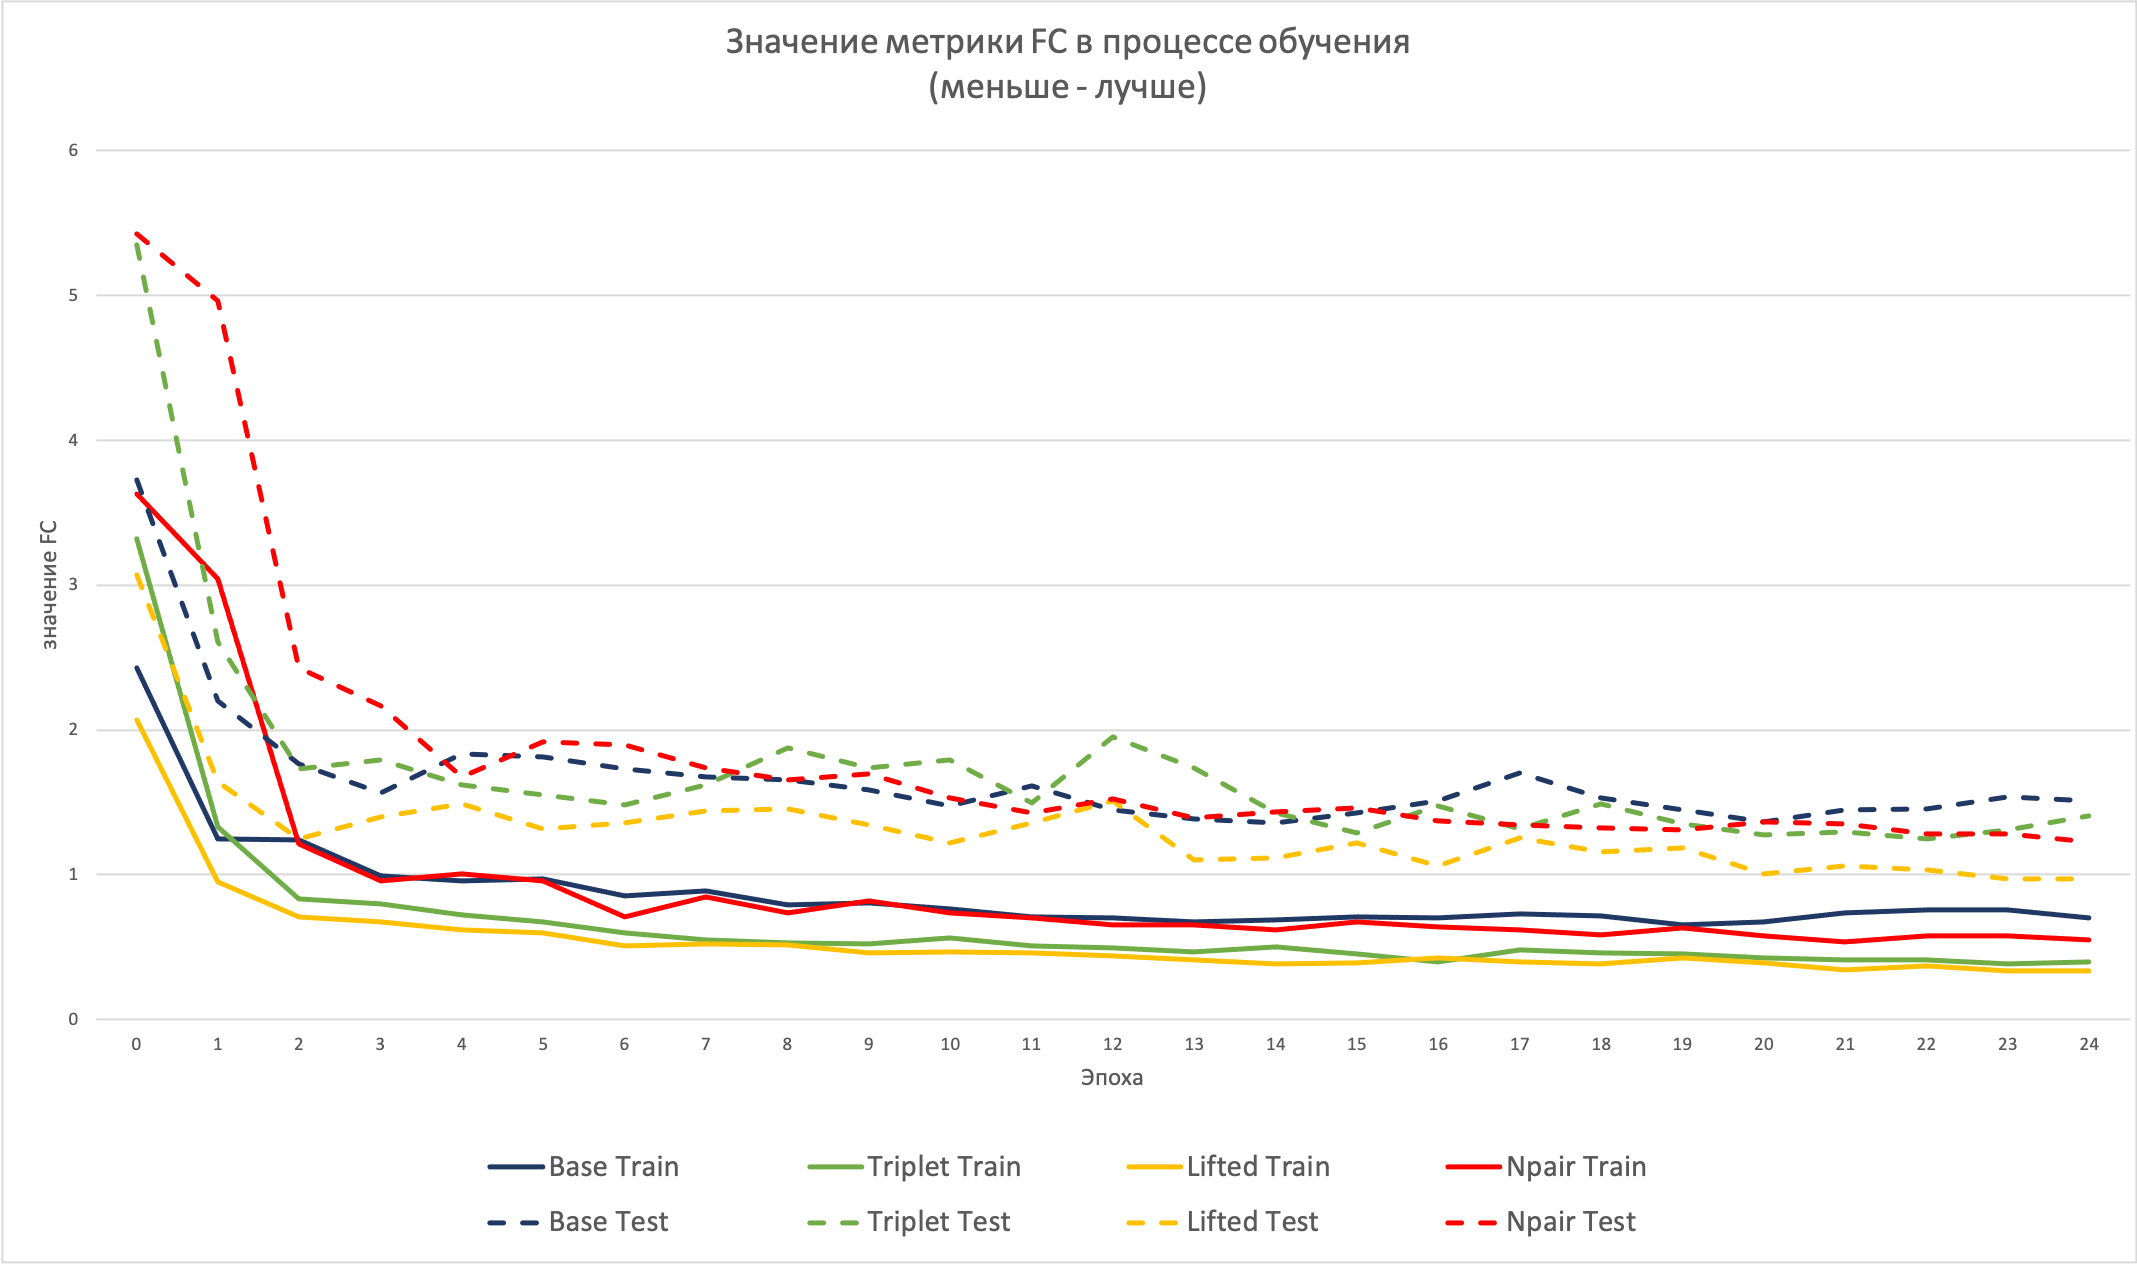
\includegraphics[width=16cm]{Images/FC_aggregate.png}
\label{fig:FC_aggregate}
\end{figure}

\begin{figure}[!h]
\caption{Изменение HV в процессе обучения}
\centering
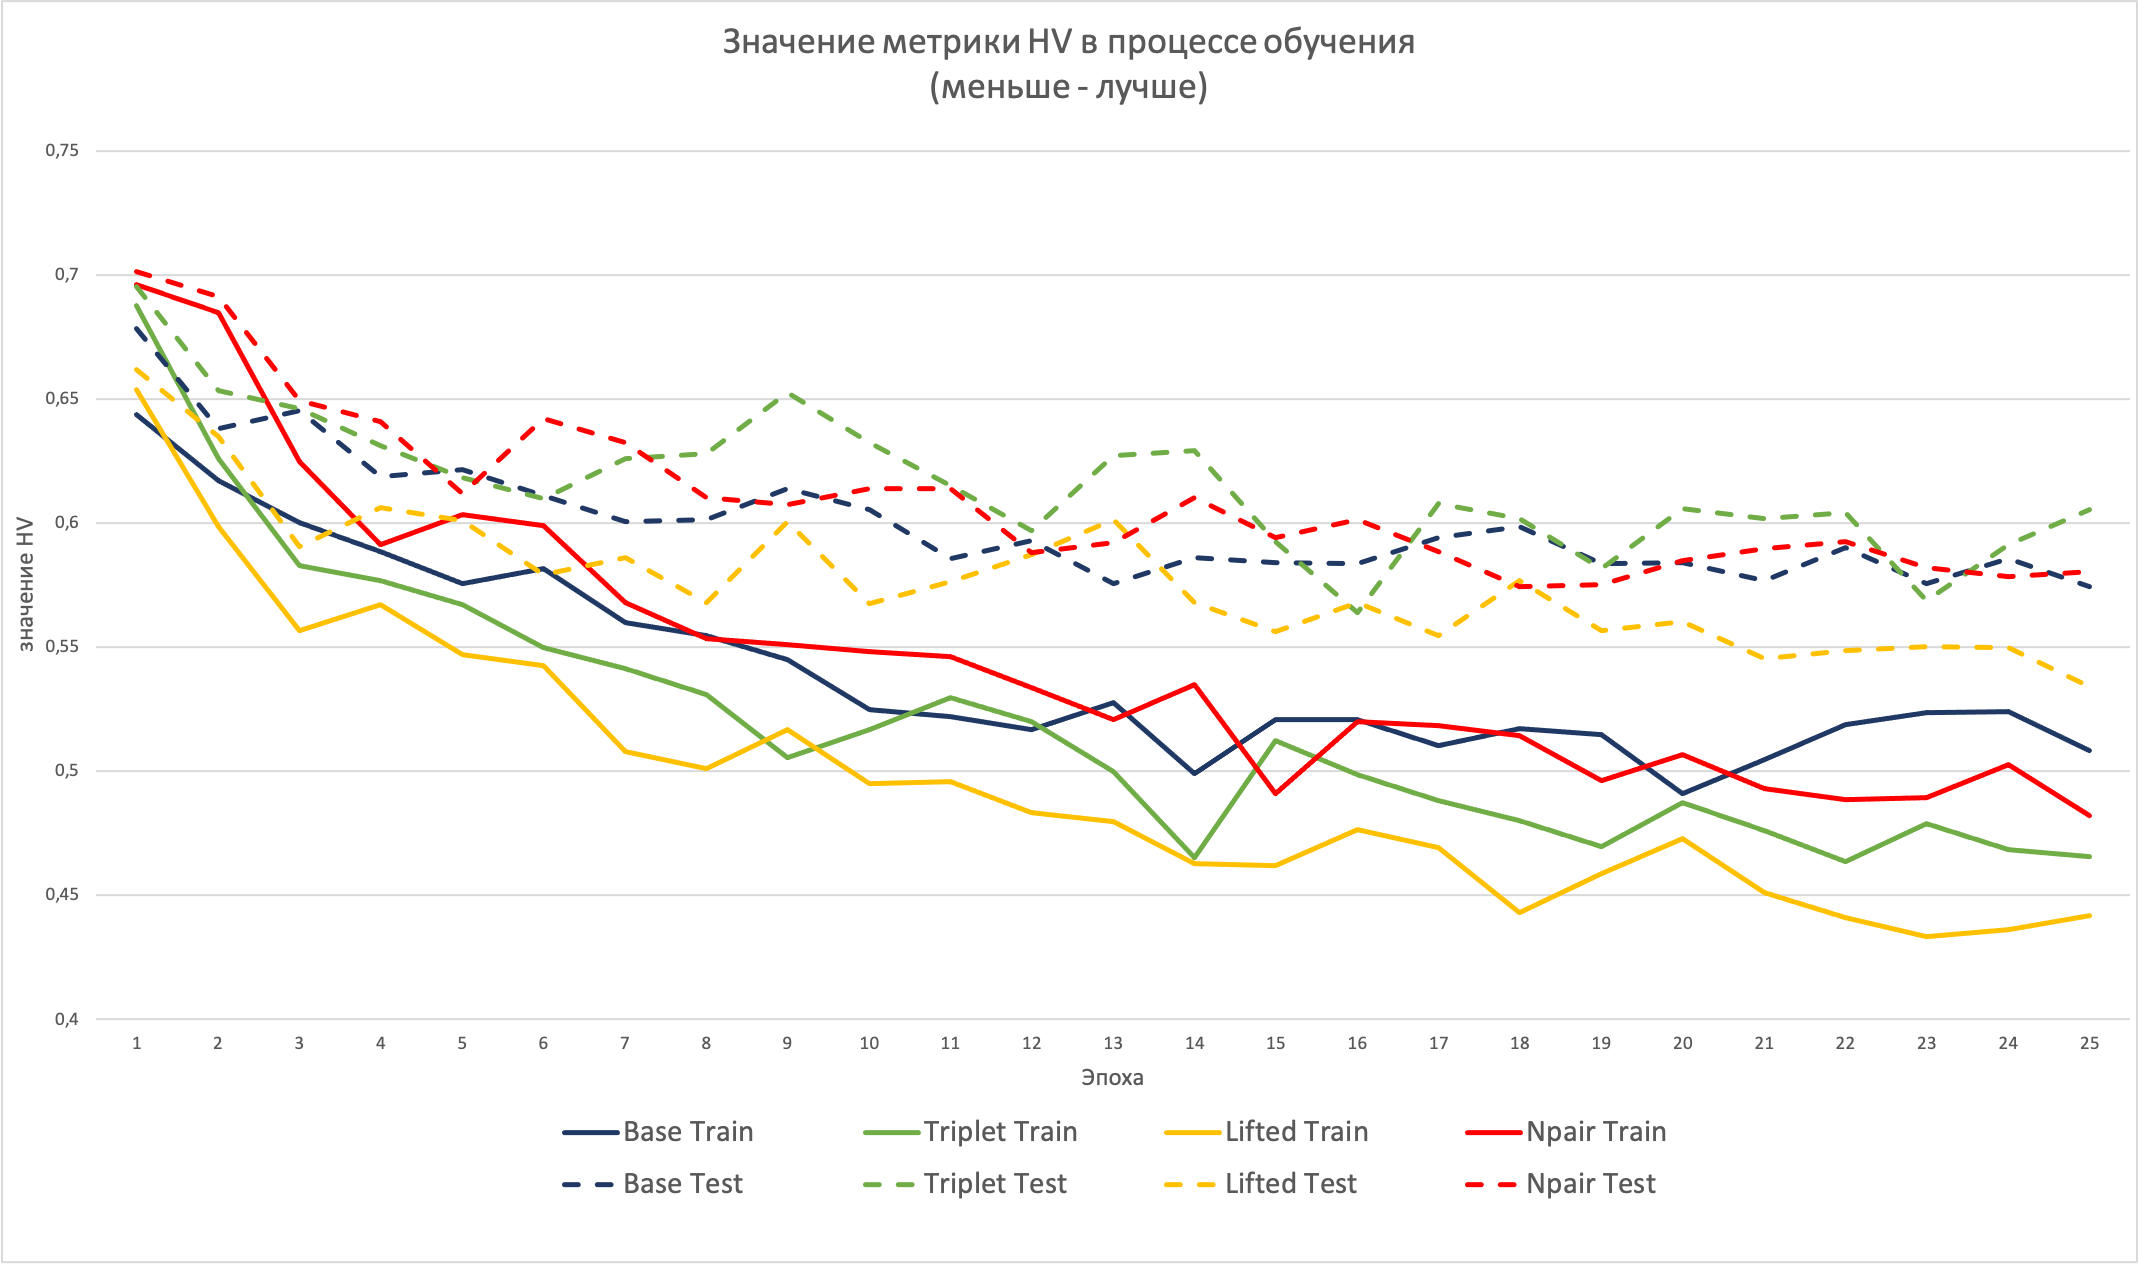
\includegraphics[width=16cm]{Images/HV_aggregate.png}
\label{fig:HV_aggregate}
\end{figure}

\par
Помимо численного подтверждения образования кластеров посредством выбранных метрик, была произведено отображение эмбеддингов в пространство размерности 2 с использованием t-SNE из бибилиотеки scikit-learn. Для проведения сравнения были выбраны по 500 случайных примеров из обучающей и тестовой выборки. На тренировочном наборе Рис.\ref{fig:tsne_train_4} видно, что во всех случаях большую часть кластеров легко выделить, однако базовая модель-классификатор и Lifted Structured Loss показали себя лучше остальных. На тестовом наборе ситуация сильно ухудшается, что ожидаемо по вычисленным ранее метрикам. Тем не менее в случае Lifted Structured Loss получились довольно плотные кластера для слов 'forward' (рыжие точки), 'go' (темно-зеленые), 'wow' (светло-голубые), 'follow' (серо-голубые), 'stop' (блекло-желтыые). Данные отобрадения дополнительно подтвердают формирование кластеров в процессе обучения с использованием описанных функций потерь, а также дает возможность изобразить превосходство использования Lifted Structured Loss.

\newpage


\begin{figure}[!h]
\caption{Применение t-SNE на тренировочном наборе}
\centering
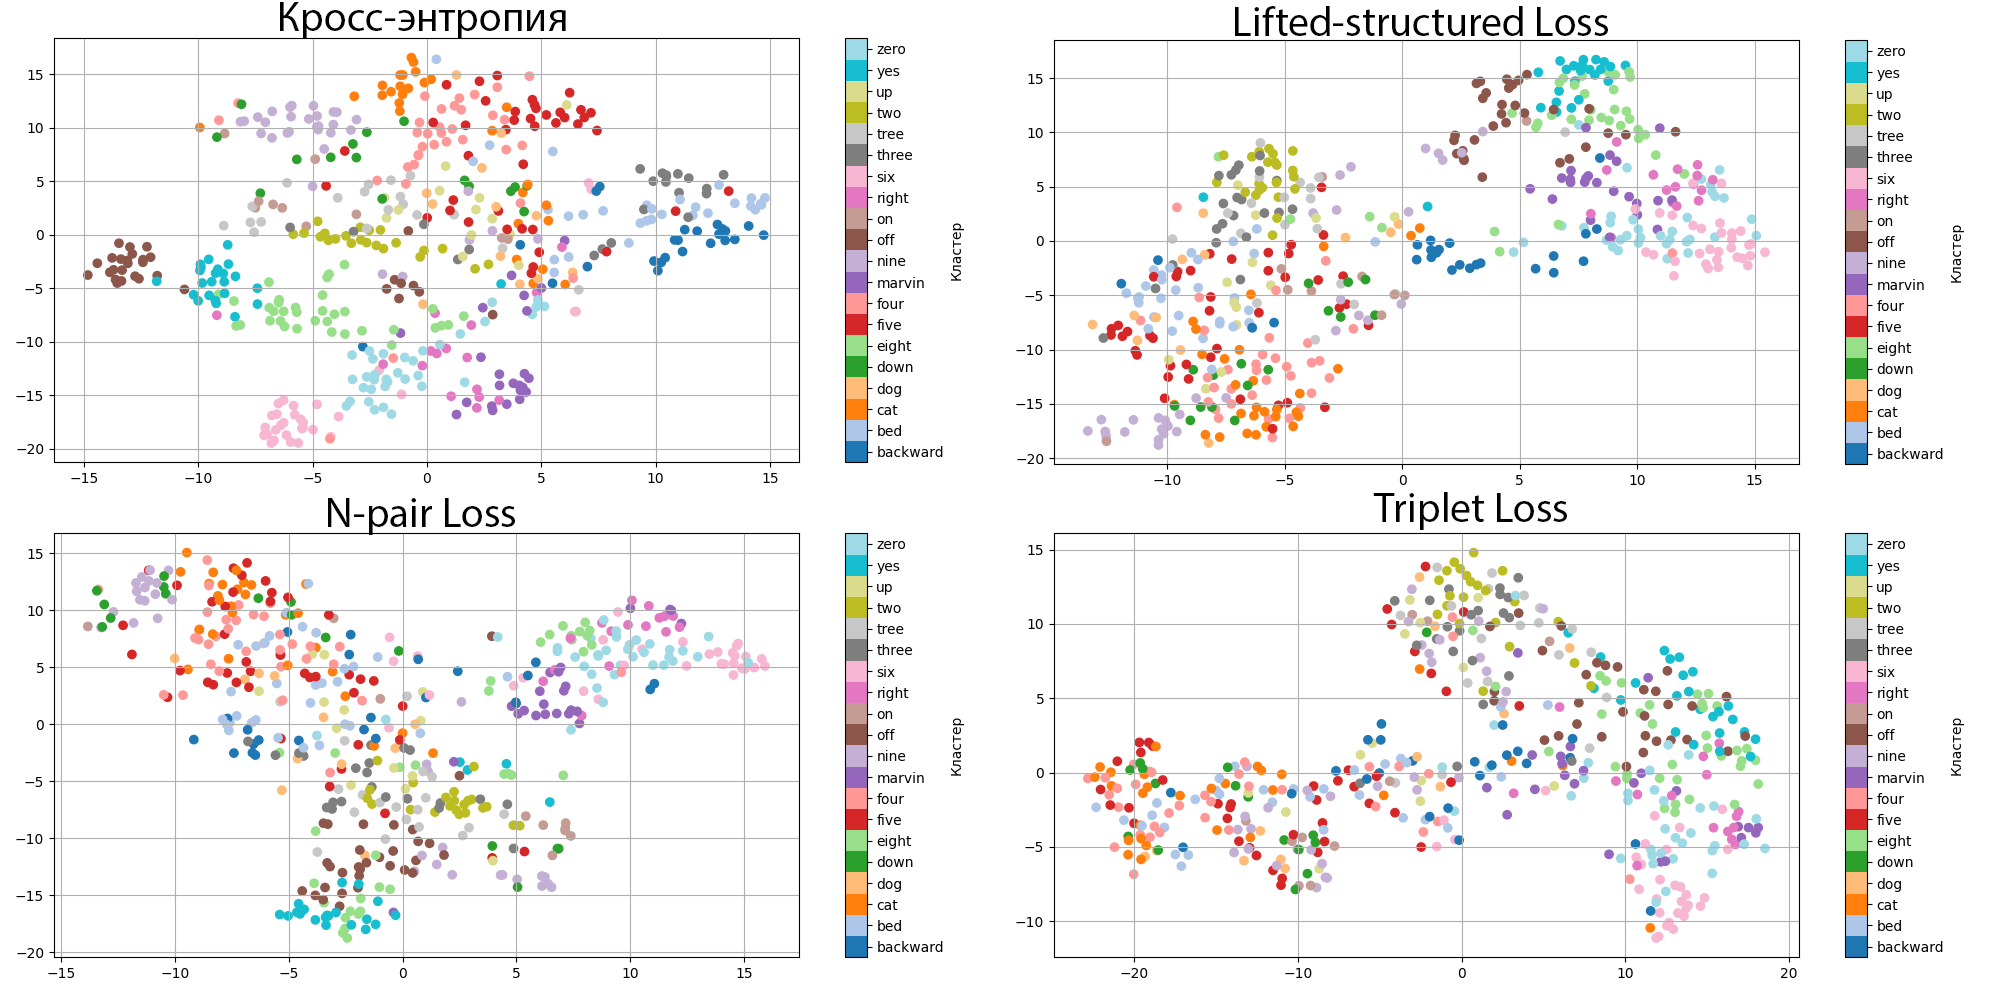
\includegraphics[width=16cm]{Images/tsne_train_4.png}
\label{fig:tsne_train_4}
\end{figure}

\begin{figure}[!h]
\caption{Применение t-SNE на тестовом наборе}
\centering
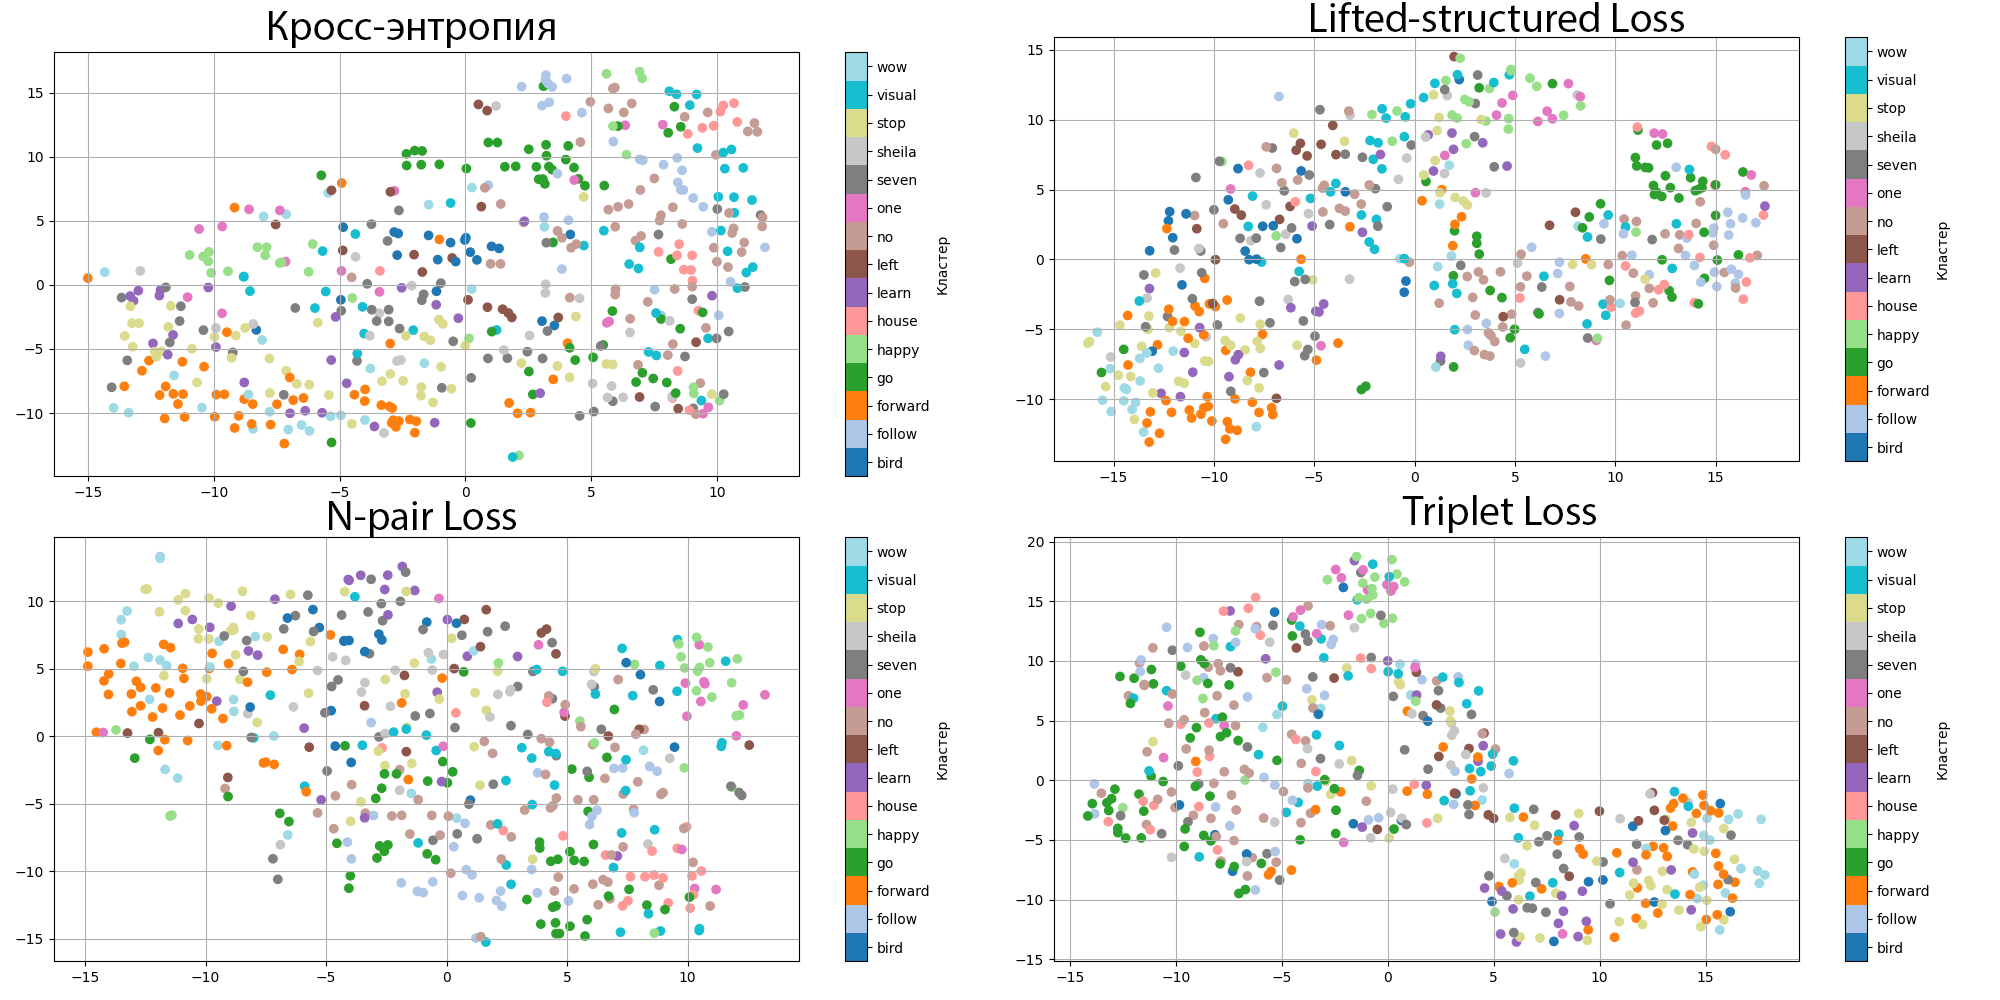
\includegraphics[width=16cm]{Images/test_tsne_4.png}
\label{fig:tsne_test_4}
\end{figure}